% 2005 年湖北卷理科第 20 题配图：四棱锥 P-ABCD 与点 E
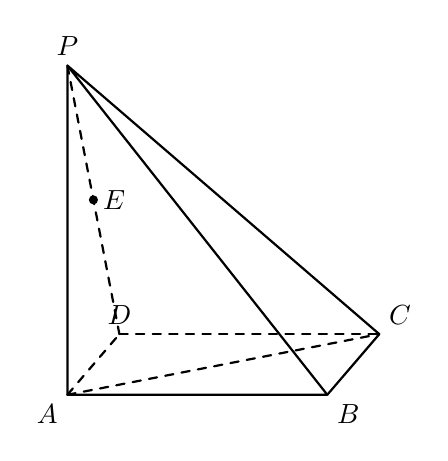
\begin{tikzpicture}[>=stealth,scale=1.1,line cap=round,line join=round]
  % 顶点坐标
  \coordinate (A) at (0,0);
  \coordinate (B) at (3.0,0);
  \coordinate (D) at (0.6,0.7);
  \coordinate (C) at (3.6,0.7);
  \coordinate (P) at (0,3.8);
  \coordinate (E) at (0.3,2.25);

  % 虚线不可见棱与对角线
  \draw[dashed,thick] (A) -- (D);
  \draw[dashed,thick] (D) -- (C);
  \draw[dashed,thick] (P) -- (D);
  \draw[dashed,thick] (A) -- (C);

  % 实线可见棱
  \draw[thick] (P) -- (A) -- (B) -- (C) -- (P) -- (B);

  % 中点 E 绘制
  \fill (E) circle (1.5pt) node[right] {$E$};

  % 顶点标签
  \node[above] at (P) {$P$};
  \node[below left] at (A) {$A$};
  \node[below right] at (B) {$B$};
  \node[above right] at (C) {$C$};
  \node[above] at (D) {$D$};
\end{tikzpicture}
